%------------ MOS Capacitances ---------------
\begin{tikzpicture}
\node [mybox] (box){%
    \begin{minipage}{0.3\textwidth}
        $C_{sb} = C_j(L_sW + x_jW) + C_{jsw}(2L_s + W)$\\
        $(L_sW + x_jW)$ is the Kang textbooks area definition, Pg. 110\\
        $C_{jsw} = C'_{jsw}x_j$\\
        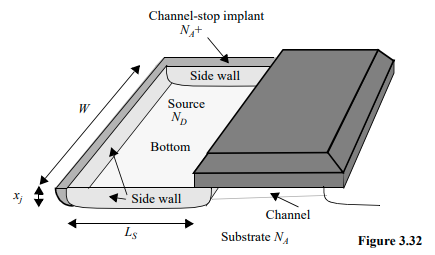
\includegraphics[scale=0.5]{sections/MOSCap.png}\\
        Pg. 112, Digital Integrated Circuits, Rabaey\\

        %\textbf{Oxide Capacitances:}\\
    	%$C_{gs} = C_{gd} = WC_o\\$
        \textbf{Junction Capacitances:}\\
        %$C_{sb} = C_{db} = C_{j} + C_{jsw}\\$
        $C_{j} = C_{jo} K_{eq}\\$
        $K_{eq} = -\frac{\phi_o^m}{(V_2 - V_1)(1-m)}[(\phi_o-V_2)^{1-m}-(\phi_o-V_1)^{1-m}]$\\
        Find $\phi_o$ in Diodes\\
        \textbf{Sidewall Capacitance}\\
        %$C_{eq(SW)} = P_{(Perimeter)}C_{josw}K_{eq(sw)}$\\
        $C'_{jsw} = C_{josw}K_{eq(sw)}$\\
        $C_{josw} = \sqrt{\frac{\epsilon_{si}q}{2}\frac{N_{a(sw)}N_d}{N_{a(sw)}+N_d}\frac{1}{\phi_{osw}}}$\\
        $K_{eq(sw)} = -\frac{2\sqrt{\phi_{osw}}}{V_2 - V_1}(\sqrt{\phi_{osw}-V_2} - \sqrt{\phi_{osw}-V_1})$\\
        $\phi_{osw} = \frac{kT}{q}ln(\frac{N_{a(sw)}N_d}{n_i^2})$\\
        $V_{to(new)} = V_{to(n)} \pm \frac{qN_i}{C_{ox}}$ Where $N_i$ is implanted carriers\\
       NMOS: $+ Acceptors, - Donors$\\
       PMOS : $+ Donors, - Acceptors$\\

       
    \end{minipage}
};
%------------ MOS Capacitances Header ---------------------
\node[fancytitle, right=10pt] at (box.north west) {MOS Capacitances};
\end{tikzpicture}